\begin{center}
    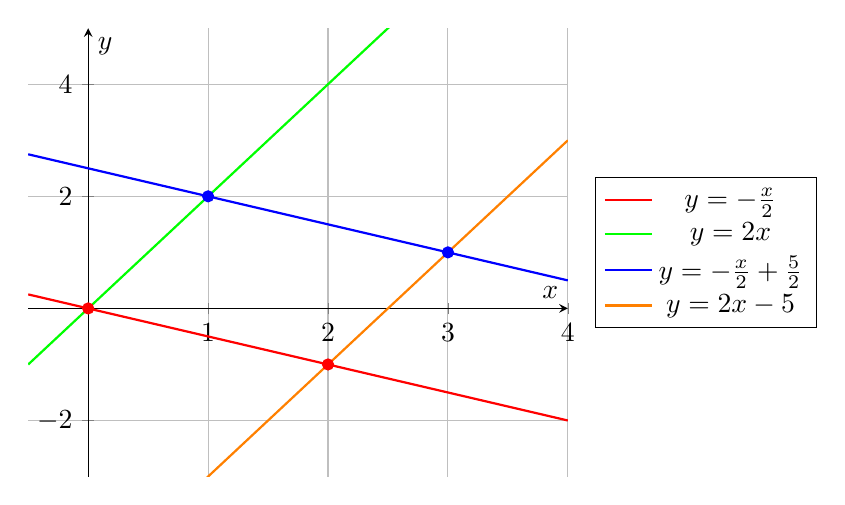
\begin{tikzpicture}
        \begin{axis}[
            axis lines = middle,
            xlabel = {$x$},
            ylabel = {$y$},
            grid = major,
            domain = -0.5:4,
            ymin = -3, 
            ymax = 5,
            legend style = {at={(1.05,0.5)}, anchor=west}
        ]
        \addplot[red, thick] {-x/2};
        \addlegendentry{$y = -\frac{x}{2}$}
        
        \addplot[green, thick] {2*x};
        \addlegendentry{$y = 2x$}
    
        \addplot[blue, thick] {-x/2 + 5/2};
        \addlegendentry{$y =-\frac{x}{2} + \frac{5}{2}$}
    
        \addplot[orange, thick] {2*x - 5};
        \addlegendentry{$y = 2x - 5$}

        \addplot[only marks, red] coordinates {(0,0) (2,-1)};
        
        \addplot[only marks, blue] coordinates {(1,2) (3,1)};
        
        \end{axis}
    \end{tikzpicture}
    \end{center}

    Obteniendo las funciones que intersecan en los puntos $(0,1),(1,0),(3,4),(4,3)$, podemos realizar el cambio de variable:
    \begin{align}
        y &= -\frac{x}{2} \\
        y &= -\frac{x}{2} + \frac{5}{2} \\
        y &= 2x \\
        y &= 2x - 5
    \end{align}

    Despejando ecuaciones semejantes:
    \[
        u = y + \frac{x}{2}, \quad v = y - 2x.
    \]    
    Donde 
    \[
        0\leq u \leq \frac{5}{2}, \quad -5 \leq v \leq 0.
    \]

    \subsection*{Transformación de variables}
    Sumando y restando las dos ecuaciones se despeja $x$ y $y$
    \[
        x = \frac{2u - 2v}{5}, \quad y = \frac{4u + v}{5}.
    \]

    \vspace{10pt}
    Por lo que llegamos a $T(u,v) = (\frac{2u - 2v}{5},\frac{4u + v}{5})$

    \subsection*{Determinante Jacobiano}
    \[
    \frac{\partial(x, y)}{\partial(u, v)}  =  \begin{vmatrix} 
        -\frac{2}{5} & \frac{2}{5} \\ \\ 
        -\frac{1}{5} & \frac{4}{5} 
    \end{vmatrix} = -\frac{8}{25} - \frac{2}{25} = -\frac{2}{5}
    \]

    Con esto:
    \begin{align*}
        \iint_D (x+y) \, dx \, dy &= \int \limits_{0}^{\frac{5}{2}} \int \limits_{-5}^{0} -\frac{2}{5}\left(\frac{2u - 2v}{5} + \frac{4u + v}{5} \right) \, du \, dv \\
        &= -\frac{2}{5} \int \limits_{0}^{\frac{5}{2}} \int \limits_{-5}^{0}\left( \frac{6u}{5} - \frac{v}{5} \right) \, du \, dv \\
        &= -\frac{2}{5} \int \limits_{0}^{\frac{5}{2}} \left[ \frac{3u^{2}}{5} - \frac{vu}{5} \right]^{0}_{-5} \, dv \\
        &= \frac{2}{5} \int \limits_{0}^{\frac{5}{2}} (v + 15) \, dv \\
        &= \frac{2}{5} \left[ \frac{v^2}{2} + 15v \right]^{\frac{5}{2}}_{0}\\
        &= \frac{2}{5} \left[\frac{325}{8}\right] \\
        &= \frac{65}{4}
    \end{align*}
